\chapter{従属化と等位接続} \label{ch:subord-coord-ja}

\epigraph{If I were a cinnamon peeler\\
I would ride your bed\\
and leave the yellow bark dust\\
on your pillow.}{Michael Ondaatje, \enquote{The Cinnamon Peeler}}

\begin{tblsframedsymbol}{学習目標}{bulb}
\begin{itemize}[noitemsep, leftmargin=*]
    \item 従属化（階層的な依存関係）と等位接続（同じ地位の要素を結ぶこと）を区別できるようになる。
    \item 複文の中で、母節、主節、従属節を見分け、分析できるようになる。
    \item 内容節、比較節、関係節という従属節の主な種類を認識できるようになる。
    \item 従属接続詞と等位接続詞が、主要部ではなく構造上の標識として機能することを理解する。
    \item 句の等位接続と節の等位接続を含め、等位構造を分析できるようになる。
    \item 複文の構造関係を判断するための診断テストを適用できるようになる。
    \item 従属化と等位接続が、文章の結束性を作るためにどのように協働するかを理解する。
    \item これらの構造が統語的な気づきを育てるうえでどのような教育的価値をもつかを理解する。
\end{itemize}
\end{tblsframedsymbol}

\section{導入}

言語によって、私たちは個々の考えだけでなく、考え同士の関係も表すことができます。そのための基本的な方法が二つあります。\term{従属化}（\term{subordination}）と\term{等位接続}（\term{coordination}）です。二つは異なる役割を担います。従属化は依存関係の階層を作り、等位接続は同じ地位の要素を結びます。

同じ基本的な考えを結ぶ次の三つの方法を見てください。

\ea \label{ex:intro-ja}
    \ea \gll Kim left. Pat came.\\
        Kim 去る-PST Pat 来る-PST\\
    \glt \trans{キムは去った。パットが来た。} [別個]
    \ex \gll The fact {\ob}that Kim left{\cb} enabled Pat's arrival.\\
        DEF 事実 Sdr Kim 去る-PST 可能にする-PST Pat-GEN 到着\\
    \glt \trans{キムが去ったという事実が、パットの到着を可能にした。} [従属]
    \ex \gll Kim left and Pat came.\\
        Kim 去る-PST and Pat 来る-PST\\
    \glt \trans{キムは去り、パットが来た。} [等位]
    \z
\z
(\ref{ex:intro-ja}a) では、二つの独立した陳述があります。(b) では、\mention{that Kim left} がより大きな構造の中に埋め込まれています。これは主語の中で補部として機能しています。(c) では、二つの節が同じ地位に置かれています。二つは同等のものとして並び、\mention{and} で結ばれているだけです。

階層と同等性のこの対比は、文法の深いところに関わります。一つの節を別の節に従属させるとき、私たちは依存関係を作っています。一つの節が、もう一方の中の要素の補部や修飾語として働くのです。要素を等位接続するときには、それらが他の点では異なっていても、構造の中では同じ地位にあると示しています。

この二種類の関係に使う道具は数が多くありません。依存関係には \mention{that} や \mention{whether} のような語が、同等性の関係には \mention{and}、\mention{or}、\mention{but} のような語が使われます。しかし、これらの小さな語によって、単純な部品から複雑な意味を作り、考え同士の関係を示し、長い推論の連鎖の中で読み手を導くことができます。これらの要素は主要部ではなく、文法的な関係を示す役割を担います。

この章では、この二つの体系が単独で、また互いに関わりながら、どのように働くかを見ていきます。従属化が、一つの考えを別の考えの中に埋め込み、意味の層を作ることを見ます。等位接続が、構造上の単純さを保ちながら複雑な考えを作る仕組みも見ます。そして、この二つの体系が互いを補い、考えられるほとんどあらゆる関係を表す柔軟性を与えてくれることを確認します。

\section{従属化}\label{sec:subordination-ja}

コミュニケーションでは、考え同士の複雑な関係を表す必要がよくあります。ある考えが別の考えに依存していることもあれば、ある考えが別の考えを修飾したり説明したりすることもあります。ここで従属化が重要になります。\term{従属化}とは、一つの節を別の構造の中の\term{従属部}（\term{dependent}）にする文法的な過程です。

\term{従属節}（\term{subordinate clause}）を含む節は\term{母節}（\term{matrix clause}）と呼ばれます。一方、それ自体を含む母節をもたない節は\term{主節}（\term{main clause}）と呼ばれます。次の例が示すように、一つの節は主節であると同時に母節でもありえます。

\ea \label{ex:sub-basic-ja}
    \ea \gll Kim left early.\\
        Kim 去る-PST 早く\\
    \glt \trans{キムは早く去った。} [主節]
    \ex \gll She thinks {[}that Kim left early{]}.\\
        she 思う-PRS {[}Sdr Kim 去る-PST 早く{]}\\
    \glt \trans{彼女はキムが早く去ったと思っている。} [従属]
    \ex \gll {[}She thinks that Kim left early{]}.\\
        {[}she 思う-PRS Sdr Kim 去る-PST 早く{]}\\
    \glt \trans{彼女はキムが早く去ったと思っている。} [主節/母節]
    \z
\z
(\ref{ex:sub-basic-ja}a) は単純な主節です。(b) では、同じ節が従属節になっています。つまり、(c) の母節の中の従属部になっています。そして (c) の母節は、同時に主節でもあります。

この型はさらに広げることができます。(\ref{ex:sub-basic2-ja}) では、(\ref{ex:sub-basic-ja}b) の節が主節から従属節に変わっていますが、それでも \mention{that Kim left} に対する母節であり続けています。つまり、一つの節は主節かつ母節でありえるだけでなく、従属節かつ母節でもありえるのです。

\ea\label{ex:sub-basic2-ja}
\gll I heard {\ob}that she thinks {\ob}that Kim left early{\cb}{\cb}.\\
    I 聞く-PST Sdr she 思う-PRS Sdr Kim 去る-PST 早く\\
\glt \trans{私は、彼女がキムは早く去ったと思っていると聞いた。} [従属]
\z

ただし、どの節も同時に\term{主節}であり\term{従属節}であることはできません。\term{母節}と\term{従属節}は関係を表す用語であり、ある節が別の節に対してどの位置にあるかを示します。一方、\term{主節}は統語的な型を表します。そして主節の構造は、さまざまな従属節の型でいつもそのまま保たれるわけではありません。

\subsection{従属節の種類}

英語には、主な有限従属節が三種類あります。\footnote{\textit{CGEL} では有限従属節と非有限従属節を区別し、その中にさまざまな種類を立てますが、ここでは扱いません。}\term{内容節}（\term{content clause}）、\term{比較節}（\term{comparative clause}）、\term{関係節}（\term{relative clause}）です。順に見ていきましょう。

\ea \label{ex:sub-types-ja}
    \ea \gll I doubt that we ordered enough books.\\
        I 疑う-PRS Sdr we 注文する-PST 十分な 本-PL\\
    \glt \trans{私たちが十分な本を注文したかどうか、私は疑っている。} [内容]
    \ex \gll More books arrived than we had ordered.\\
        より多い 本-PL 届く-PST than we 注文する-PST\\
    \glt \trans{私たちが注文したより多くの本が届いた。} [比較]
    \ex \gll The books that we ordered arrived.\\
        DEF 本-PL Rel we 注文する-PST 届く-PST\\
    \glt \trans{私たちが注文した本が届いた。} [関係]
    \z
\z
内容節は既定の型です。関係節や比較節がもつ特別な統語的性質をもっていません。関係節は次の章の中心的な話題なので、ここではまず内容節を見て、それから比較節を扱います。

\subsubsection{内容節}

内容節には大きく二つの種類があります。(\ref{ex:content-types-ja}) のような平叙節と疑問節です。\footnote{\textit{CGEL} では感嘆の内容節も扱われますが、かなりまれです。}

\ea \label{ex:content-types-ja}
    \ea \gll She said that it was genuine.\\
        she 言う-PST Sdr it である-PST 本物\\
    \glt \trans{彼女はそれが本物だと言った。} [平叙]
    \ex \gll She asked whether it was genuine.\\
        she 尋ねる-PST whether it である-PST 本物\\
    \glt \trans{彼女はそれが本物かどうか尋ねた。} [基本疑問]
    \ex \gll She asked what made it genuine.\\
        she 尋ねる-PST what する-PST it 本物\\
    \glt \trans{彼女は何がそれを本物にしているのか尋ねた。} [焦点化疑問]
    \z
\z
(\ref{ex:content-types-ja}a と b) の \mention{that} と \mention{whether} は重要な働きをしています。それぞれの節が従属していることを標示しているのです。ここで、新しいが非常に小さなカテゴリーである\term{従属接続詞}（\term{subordinator}, Sdr）が出てきます。このカテゴリーの主な成員は \mention{that} と \mention{whether}、そして `whether' の意味の \mention{if} です。条件を表す \mention{if} ではありません。従属接続詞は特別です。他の語彙範疇と違い、句を投射しないからです。名詞にはNPがあり、動詞にはVPがありますが、従属接続詞にはSdrPがありません。その代わり、従属接続詞は純粋に標識として働き、その節がより大きな構造とどう関係するかを示します。木構造は図~\ref{fig:sub-tree-sub-ja}に示しています。（三角形は、一部の構造が省略されていることを表します。第6章を参照してください。）

\begin{figure}
    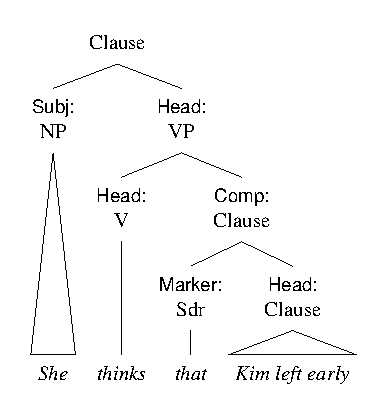
\includegraphics[width=0.55\linewidth]{figures/she thinks that kim left.pdf}
    \caption{従属化を示す統語木：\mention{She thinks that Kim left early} において、\mention{that Kim left early} が補部として機能している}\label{fig:sub-tree-sub-ja}
\end{figure}

従属構造では、\mention{that} が標識として現れていることに注意してください。\mention{that} は自分自身の句を投射しているのではなく、従属節の始まりを示しているだけです。\term{標識}（\term{marker}, Mk）とは、主要部がより大きな構造と文法的にどのように関係するかを示す従属部の一種です。

内容節は、より大きな構造の中でさまざまな働きをします。

\ea \label{ex:content-funcs-ja}
    \ea \gll I suspect {\ob}that he left{\cb}.\\
        I 疑う-PRS Sdr he 去る-PST\\
    \glt \trans{私は彼が去ったのではないかと思っている。} [VP内]
    \ex \gll The fact {\ob}that he left{\cb} is clear.\\
        DEF 事実 Sdr he 去る-PST である-PRS 明らか\\
    \glt \trans{彼が去ったという事実は明らかだ。} [NP内]
    \ex \gll I'm glad {\ob}that he left{\cb}.\\
        I-である 嬉しい Sdr he 去る-PST\\
    \glt \trans{彼が去ってくれて私はうれしい。} [AdjP内]
    \ex \gll We can proceed provided {\ob}that he left{\cb}.\\
        we できる-PRS 進む provided Sdr he 去る-PST\\
    \glt \trans{彼が去ったのであれば、私たちは先に進める。} [PP内]
    \ex \gll Whether or not he left is unclear.\\
        whether or not he 去る-PST である-PRS 不明\\
    \glt \trans{彼が去ったかどうかは不明だ。} [主語]
    \ex \gll It's unclear whether or not he left.\\
        it-である 不明 whether or not he 去る-PST\\
    \glt \trans{彼が去ったかどうかは不明だ。} [外置主語]
    \z
\z

平叙内容節では、標識、つまり従属接続詞 \mention{that} は、その節の機能によって、必須であったり、任意であったり、許されなかったりします。
\ea\label{ex:marker-need-ja}
    \ea \gll That Kim left surprised no one.\\
        Sdr Kim 去る-PST 驚かせる-PST 誰も-ない\\
    \glt \trans{キムが去ったことは誰も驚かせなかった。} [必須]
    \ex \gll I know that Kim left.\\
        I 知る-PRS Sdr Kim 去る-PST\\
    \glt \trans{私はキムが去ったことを知っている。} [任意]
    \ex \gll *We left before that Kim arrived.\\
        *we 去る-PST before Sdr Kim 到着する-PST\\
    \glt \trans{意図された意味：私たちはキムが到着する前に去った。英語ではここで \mention{that} は使えない。} [*; 不可]
\z
\z
(\ref{ex:marker-need-ja}a) のような主語節では、標識が常に必要です。補部として働く場合、平叙節は (b) のように、たいてい標識があってもなくてもかまいません。主な例外は、(c) のようにPP内の補部として働く場合です。

\label{sec:sub-interrog-ja}

疑問内容節は興味深いものです。主節の疑問節とは統語的に異なるからです。主節の基本疑問節は、\mention{Did she accept?} のような主語・助動詞倒置で見分けることができます。一方、その従属節版は、疑問であることを \mention{whether} や \mention{if} で示します。

\ea 基本疑問節\label{ex:int-sub-ja}
    \ea \gll Did she accept?\\
        AUX she 受け入れる\\
    \glt \trans{彼女は受け入れたのか。} [主節、倒置]
    \ex \gll I wonder {\ob}whether she accepted{\cb}.\\
        I 思う-PRS whether she 受け入れる-PST\\
    \glt \trans{私は彼女が受け入れたかどうか気になっている。} [従属]
    \z
\z
\ea 焦点化疑問節
    \ea \gll How did we get here?\\
        how AUX we 来る ここへ\\
    \glt \trans{私たちはどうやってここに来たのか。} [主節、倒置]
    \ex \gll I wonder {\ob}how we got here{\cb}.\\
        I 思う-PRS how we 来る-PST ここへ\\
    \glt \trans{私は私たちがどうやってここに来たのか気になっている。} [従属]
    \z
\z
これは英語学習者にとって難しい点です。初級者はたいてい何も倒置せず、主節の疑問節を誤って作ります。もう少し経験のある学習者は、倒置を理解したために、それをどこにでも適用し、従属疑問節を誤って構造化してしまいます。この区別を楽に扱えるようになるのは、かなり高いレベルになってからです。

とはいえ、主節の疑問節と従属疑問節の構造上の違いは、少しずつ崩れ始めています。倒置がゆっくり拡大し続けているからです。書き言葉で倒置した疑問内容節を見ることはまだまれですが、(\ref{ex:non-inverted-interrogative-ja}) のような例は話し言葉ではかなり一般的になっています。数百年後には、すべての疑問節で倒置が標準になり、標識が任意になるかもしれません。私は待つつもりはありません。

\ea\label{ex:non-inverted-interrogative-ja}
\gll We need a story of {\ob}how did we get here{\cb}.\\
    we 必要とする-PRS a 物語 of how AUX we 来る ここへ\\
\glt \trans{私たちは、どうやってここに来たのかという物語を必要としている。}
\z
しかし今のところ、基本疑問の内容節では、通常 \mention{whether} や \mention{if} のような標識が常に必須です。そうでなければ、ほとんどの場合、標識のない平叙節と区別できなくなってしまいます。

\subsubsection*{mandative構文}

従属構文の特殊な下位型に、\term{mandative構文}があります。これは、要求や必要性を表す述語とともに現れます。

\ea \label{ex:mandative-ja}
    \ea \gll It is essential {\ob}that he be there{\cb}.\\
        it である-PRS 必須 Sdr he いる-PLAIN そこに\\
    \glt \trans{彼がそこにいることが不可欠だ。} [仮定法現在]
    \ex \gll It is essential {\ob}that he should be there{\cb}.\\
        it である-PRS 必須 Sdr he should いる そこに\\
    \glt \trans{彼がそこにいるべきだということが不可欠だ。} [should]
    \ex \gll It is essential {\ob}that he is there{\cb}.\\
        it である-PRS 必須 Sdr he いる-PRS そこに\\
    \glt \trans{彼がそこにいることが不可欠だ。} [直説法]
    \z
\z
\term{仮定法現在}（\term{present subjunctive}）の変種では、動詞の原形が使われます。ここでの「仮定法」は反事実を表しているという意味ではありません。英語の \mention{that he be there} で重要なのは、要求や必要性の文脈で \mention{be} という原形が現れていることです。\mention{should} 型は、少なくとも以前は、イギリス英語でより一般的でした。アメリカ英語では仮定法現在が好まれる傾向があります。\term{直説法}（\term{indicative}）の変種では、通常の時制をもつ形が使われます。

これは、従属節の中の変異が微妙な意味の違いや地域的な好みを示しうることをよく示す例です。教育上は、直説法の形が、特にくだけた文脈では、より一般的になりつつあることを指摘しておく価値があります。ただし、形式的な書き言葉では仮定法現在が今でも標準的です。

\begin{tblsframedsymbol}{理解確認：母節と従属節}{test}
構造関係を見分ける練習をしましょう。
\begin{itemize}[noitemsep, leftmargin=*]
    \item \mention{I know that she thinks that he left} で、主節、母節、従属節を見つけてください。
    \item \mention{She asked whether he left} には倒置がないのに、\mention{Did he leave?} には倒置がある理由を説明してください。
    \item mandative構文を見つけてください：\mention{It's important that he be careful} と \mention{It's important that he is careful}。
\end{itemize}
こうした構造関係を理解すると、意味が統語的な構造からどのように生じるかが見えやすくなります。
\end{tblsframedsymbol}

\subsection{比較節}

有限従属節の第二の主要な型は比較節です。比較節は、(\ref{ex:comparative-intro-ja}) のように、比較を完成させる節です。

\ea \label{ex:comparative-intro-ja}
    \ea \gll The ice was thicker than {\ob}we expected{\cb}.\\
        DEF 氷 である-PST より厚い than we 予想する-PST\\
    \glt \trans{氷は私たちが予想したより厚かった。}
    \ex \gll She writes faster than {\ob}she speaks{\cb}.\\
        she 書く-PRS より速く than she 話す-PRS\\
    \glt \trans{彼女は話すより速く書く。}
    \ex \gll It doesn't cost as much as {\ob}I'd thought{\cb}.\\
        it NEG かかる-PRS as 多く as I-思う-PST\\
    \glt \trans{それは私が思っていたほど高くない。}
    \z
\z
比較節を内容節から区別するのは、比較節には省略が含まれるという点です。文脈から回復できる要素が外に出されます。(\ref{ex:comparative-ellipsis-ja}) では、\dots が省略を示しています。\footnote{以前の章で空所を導入しました。空所は木の中にある構造上の位置です。一方、省略は文脈から意味的に回復できる素材ですが、統語的な要素として存在するわけではありません。}

\ea \label{ex:comparative-ellipsis-ja}
    \ea \gll Kim read more books than {\ob}Pat read \dots{\cb}.\\
        Kim 読む-PST より多い 本-PL than Pat 読む-PST \dots\\
    \glt \trans{キムはパットが読んだより多くの本を読んだ。}
    \ex \gll Kim read more books than {\ob}Pat did \dots{\cb}.\\
        Kim 読む-PST より多い 本-PL than Pat AUX.PST \dots\\
    \glt \trans{キムはパットより多くの本を読んだ。}
    \ex \gll Kim read more books than {\ob}Pat{\cb}.\\
        Kim 読む-PST より多い 本-PL than Pat\\
    \glt \trans{キムはパットより多くの本を読んだ。}
    \z
\z

最初の二つの変種は省略を示しています。(b) では \mention{read} を繰り返す代わりに、VPの代用形式である \mention{did} が使われています。三つ目の (c) では、\mention{Pat} は節の補部ではなくNP補部です。三つは基本的に同じ意味です。

多くの省略の場合と違い、比較節では省略された情報を明示すると非文法的になります。たとえば、*\mention{Kim read more books than Pat read 20 books} や *\mention{It's not as deep as it is 20 cm wide} は言えません。省略はこの節の型の重要な一部です。比較節の構造は図~\ref{fig:comp-tree-ja}に示されています。

\begin{figure}
    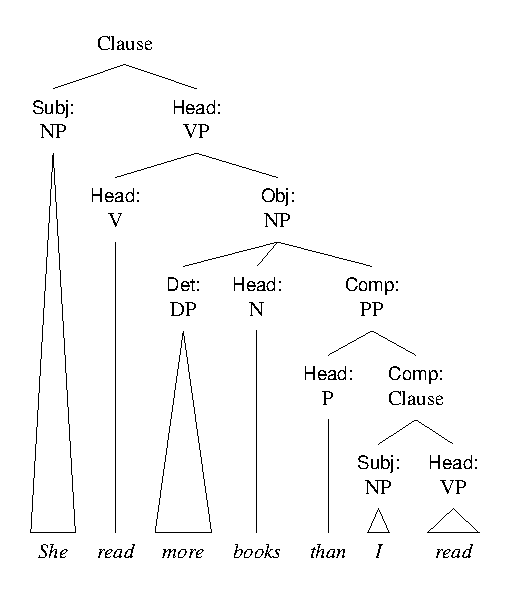
\includegraphics[width=0.7\linewidth]{figures/she read more books than I read.pdf}
    \caption{省略を伴う比較節を示す統語木}\label{fig:comp-tree-ja}
\end{figure}

比較節は、比較の種類に応じて、\mention{than} または \mention{as} をもつPPの中で補部として機能します。

\ea \label{ex:comp-markers-ja}
    \ea \gll Kim is taller than {\ob}Pat is{\cb}.\\
        Kim である-PRS より背が高い than Pat である-PRS\\
    \glt \trans{キムはパットより背が高い。} [不等]
    \ex \gll Kim is as tall as {\ob}Pat is{\cb}.\\
        Kim である-PRS as 背が高い as Pat である-PRS\\
    \glt \trans{キムはパットと同じくらい背が高い。} [同等\footnote{ここでの\emph{同等}という語は少し誤解を招くかもしれません。この例は、キムが少なくともパットと同じくらい背が高いという意味で、キムのほうが高い可能性もあります。}]
    \z
\z
(\ref{ex:comp-markers-ja}a) の \mention{than} は不等を表し、(b) の \mention{as} は同等を標示します。最初の \mention{as} は副詞です。\mention{as tall} というAdjPがあり、その中で \mention{as} は修飾語として働きます。二つ目の \mention{as} は前置詞です。

英語学習者にとって、比較節にはいくつかの難しさがあります。
\begin{itemize}[noitemsep]
    \item 何を、いつ、どれだけ省略できるのかを理解すること。
    \item 同等と不等の異なる型を習得すること。
    \item 複数の要素が関わる複雑な比較を扱うこと。
\end{itemize}

よい知らせは、比較節はかなり規則的な型に従うということです。学習者は、より複雑な構造に進む前に、\mention{taller than} `...より背が高い' や \mention{as tall as} `少なくとも...と同じくらい背が高い' のような基本的な形を習得できます。

\section{等位接続}\label{sec:coordination-ja}

従属化が節同士の依存関係を作るのに対して、\term{等位接続}は同じ統語的地位をもつ要素を結びます。この体系の中心には、\term{等位接続詞}（\term{coordinator}, Crd）と呼ばれる小さな閉じた語類があります。主なものは \mention{and}、\mention{or}、\mention{but} です（三つを列挙するだけでも三つすべてが必要です）。従属接続詞と同じく、等位接続詞も標識として機能します。

ここでの\term{等位接続}は、単に要素を「並べる」ことではありません。日本語の「並列」は説明の手がかりにはなりますが、この章で必要なのは、二つ以上の要素が同じ統語的地位をもち、どれも全体の主要部ではないという構造上の関係です。この点を忘れると、等位接続をただのリストや談話上のつながりと取り違えやすくなります。

次の例を見てください。

\ea \label{ex:coord-basic-ja}
    \ea \gll {\ob}Jane is a good teacher{\cb} {\ob}and her students really like her{\cb}.\\
        Jane である-PRS a 良い 教師 and her 学生-PL 本当に 好む-PRS her\\
    \glt \trans{ジェーンはよい教師で、学生たちは彼女を本当に好いている。}
    \ex \gll They offered us a choice of {\ob}red wine{\cb}, {\ob}white wine{\cb}, {\ob}or beer{\cb}.\\
        they 提供する-PST us a 選択 of 赤 ワイン 白 ワイン or ビール\\
    \glt \trans{彼らは赤ワイン、白ワイン、またはビールという選択肢を私たちに示した。}
    \ex \gll Her assistant is {\ob}very young{\cb} {\ob}but a quick learner{\cb}.\\
        her 助手 である-PRS とても 若い but a 速い 学習者\\
    \glt \trans{彼女の助手はとても若いが、覚えが早い。}
    \z
\z
これらの例で該当する要素は、\term{等位要素}（\term{coordinate}）として機能しています。この機能は、(\ref{ex:coord-basic-ja}a) のような節、(b) のようなNPや他の句、またよりまれには (c) のAdjPとNPのようなカテゴリーの混在によって実現されます。等位接続詞は通常、それぞれ異なる関係を表します。\mention{and} は追加、\mention{or} は選択肢、\mention{but} は対比を表します。

等位接続がこれまで見てきた構造と異なるのは、主要部をもたないという点です。どの等位要素も、構造全体の主要部ではありません。この主要部のなさは、単純なテストで見えます。多くの場合、等位接続全体を、どちらか一つの等位要素で置き換えることができます。

\ea \label{ex:coord-replace-ja}
    \ea \gll Her assistant is very young.\\
        her 助手 である-PRS とても 若い\\
    \glt \trans{彼女の助手はとても若い。}
    \ex \gll Her assistant is a quick learner.\\
        her 助手 である-PRS a 速い 学習者\\
    \glt \trans{彼女の助手は覚えが早い。}
    \z
\z
(\ref{ex:coord-replace-ja}a) と (b) はどちらも、(\ref{ex:coord-basic-ja}c) の文法的な代替になります。これは \mention{very young} のような主要部をもつ構造とはかなり違います。その場合、主要部だけなら使えます（\mention{she's young}）が、従属部だけは使えません（*\mention{she's very}）。等位接続の構造は図~\ref{fig:coord-basic-ja}に示されています。

\begin{figure}
    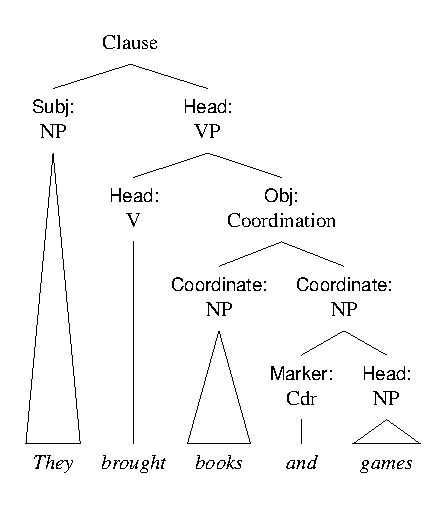
\includegraphics[width=0.65\linewidth]{figures/the brought books and games.pdf}
    \caption{標識を伴う基本的な等位接続：\mention{They brought books and games}}\label{fig:coord-basic-ja}
\end{figure}

\subsection{等位接続の性質}

三つの重要な性質が、等位接続を他の構造から区別します。

等位要素の数には文法上の制限がありません。\mention{but} は例外です。

\ea \label{ex:coord-multiple-ja}
\gll Nothing noble, sublime, profound, delicate, tasteful or even decent can find a place.\\
    何も 高貴な 崇高な 深い 繊細な 趣味のよい or さえ まともな できる-PRS 見つける 場所\\
\glt \trans{高貴なもの、崇高なもの、深いもの、繊細なもの、趣味のよいもの、まともなものでさえ、居場所を見つけることはできない。}
\z

等位要素は機能的に似ていなければなりません。単独で使ったときに、同じ機能を果たせる必要があります。

\ea \label{ex:coordinate-function-ja}
    \ea \gll I'll be back next week or at the end of the month.\\
        I-FUT 戻る 来週 or at DEF 終わり of DEF 月\\
    \glt \trans{私は来週、または月末に戻る。} [時間の付加部]
    \ex \gll *We're leaving Rome and next week.\\
        *we-PRS 去る Rome and 来週\\
    \glt \trans{意図された構造は英語では不自然である。\mention{Rome} は目的語だが、\mention{next week} は付加部である。} [*; 目的語と付加部]
    \z
\z

拡張された等位要素、つまり等位接続詞を含む等位要素は、前に移動できません。

\ea \label{ex:coord-front-ja}
    \ea \gll They attended but they aren't members.\\
        they 出席する-PST but they NEG-である-PRS 会員-PL\\
    \glt \trans{彼らは出席したが、会員ではない。}
    \ex \gll *But they aren't members, they attended.\\
        *but they NEG-である-PRS 会員-PL they 出席する-PST\\
    \glt \trans{意図された意味：彼らは出席したが、会員ではない。英語では、\mention{but} を伴う拡張等位要素をこのように前に出すことはできない。} [*]
    \z
\z

\subsection{文頭の等位接続詞について}

\mention{and} や \mention{but} のような等位接続詞で文を始めてはいけない、という規範的な規則があります。しかし、この禁止には英語の文法や用法に根拠がありません。文頭の等位接続詞は、英語史を通じて優れた書き手に使われてきました。この本でも、この章や他の章で多くの例が見つかります。ただし、文頭の等位接続詞は、その文を前の文と狭い意味での等位接続にすることはできません。(\ref{ex:coord-front-ja}) の前置制限を思い出してください。その代わりに、\term{談話接続表現}（\term{discourse connector}）として働き、新しい文が前の内容とどう関係するかを示すことができます。

ここが日本語読者にとって特に混同しやすい点です。談話接続表現は文章の流れをつなぐものです。一方、この章でいう等位接続は、一つの統語構造の内部で同じ地位の要素を結ぶものです。唯一の本当の制約は文体上のものです。どんな道具でもそうですが、文頭の等位接続詞も使いすぎれば単調になります。慎重に使えば、談話の流れを管理し、テキスト内の関係を示す有効な手段です。

\subsection{等位接続の種類}

もっとも単純な区別は、\term{対称的等位接続}（\term{symmetric coordination}）と\term{非対称的等位接続}（\term{asymmetric coordination}）の区別です。対称的等位接続では等位要素の順序は意味に影響しませんが、非対称的等位接続では影響します。

\ea \label{ex:coord-sym-ja}
    \ea \gll I was hungry and tired.\\
        I である-PST 空腹 and 疲れた\\
    \glt \trans{私は空腹で疲れていた。} [対称的]
    \ex \gll I got up and had breakfast.\\
        I 起きる-PST and とる-PST 朝食\\
    \glt \trans{私は起きて朝食をとった。} [非対称的]
    \z
\z
(\ref{ex:coord-sym-ja}a) では、等位要素の順序を逆にしても意味は変わりません。しかし (b) では、順序が時間的な連続を含意します。起きることが朝食の前に起こったのです。

\term{分配的等位接続}（\term{distributive coordination}）と\term{共同的等位接続}（\term{joint coordination}）も区別します。

\ea \label{ex:coord-dist-ja}
    \ea \gll Kim and Pat are fine players.\\
        Kim and Pat である-PRS 良い 選手-PL\\
    \glt \trans{キムとパットは優れた選手だ。} [分配的]
    \ex \gll Kim and Pat are a good pair.\\
        Kim and Pat である-PRS a 良い ペア\\
    \glt \trans{キムとパットはよいペアだ。} [共同的]
    \z
\z
(\ref{ex:coord-dist-ja}a) では、優れた選手であるという性質がキムとパットそれぞれに当てはまります。しかし (b) では、よいペアであるという性質は二人一緒の場合にだけ当てはまります。どちらか一人だけではペアにはなれません。

\subsection{等位接続の標示}

等位接続はいくつかの方法で標示できます。
\begin{itemize}[noitemsep]
    \item 等位接続詞を使う：\mention{red and blue}
    \item 標識を使わない：\mention{red, white, blue}
    \item 等位接続詞を繰り返す：\mention{red or white or blue}
    \item 相関的な標識を使う：\mention{both red and blue}
\end{itemize}

等位接続詞は通常、追加（\mention{and}）、選択肢（\mention{or}）、対比（\mention{but}）を表しますが、非対称的等位接続では追加の意味を担うこともあります。

\ea \label{ex:coord-meaning-ja}
    \ea \gll Pay within a week and you'll get a discount.\\
        支払う within a 週 and you-FUT 得る a 割引\\
    \glt \trans{一週間以内に支払えば、割引を受けられる。} [条件]
    \ex \gll Pay within a week or you'll lose the discount.\\
        支払う within a 週 or you-FUT 失う DEF 割引\\
    \glt \trans{一週間以内に支払わなければ、割引を失う。} [否定条件]
    \z
\z

\begin{tblsframedsymbol}{パターン認識：等位接続か従属化か}{test}
次の構造を区別するために、診断テストを使ってください。
\begin{itemize}[noitemsep, leftmargin=*]
    \item \mention{She thinks that he left} と \mention{She left and he stayed}: どちらが一つの節を別の節の中に埋め込み、どちらが同じ地位の二つの節を結んでいますか。
    \item \mention{Although it rained, we went} と \mention{It rained but we went}: どちらが依存関係の階層を示し、どちらが同じ地位を示していますか。
    \item \mention{*But we went, it rained} と \mention{Although it rained, we went}: 前置は構造について何を示していますか。
\end{itemize}
これらのテストは、階層的な埋め込みと、同じ地位の要素を結ぶことを区別する助けになります。
\end{tblsframedsymbol}

等位接続詞を導入したことで、間投詞を除き、英語の主要な語彙範疇をすべて見たことになります。また、それらが節の中で果たす主な統語機能にも出会ったことになります。

\subsection{等位接続の構造}

要素を等位接続するとき、それらは同じ統語機能を共有していなければなりません。つまり、補部同士や修飾語同士は等位接続できますが、補部と修飾語は等位接続できません。比べてください。

\ea \label{ex:coord-function-ja}
    \ea \gll We listened {\ob}to the teacher{\cb} {\ob}and the students{\cb}.\\
        we 聞く-PST to DEF 教師 and DEF 学生-PL\\
    \glt \trans{私たちは教師と学生たちの話を聞いた。} [補部]
    \ex \gll We listened {\ob}Monday{\cb} and {\ob}Tuesday{\cb}.\\
        we 聞く-PST 月曜 and 火曜\\
    \glt \trans{私たちは月曜と火曜に聞いた。} [修飾語]
    \ex \gll *We listened {\ob}to the teachers{\cb} and {\ob}Monday{\cb}.\\
        *we 聞く-PST to DEF 教師-PL and 月曜\\
    \glt \trans{意図された構造は英語では不自然である。\mention{to the teachers} は補部だが、\mention{Monday} は修飾語である。} [*; 機能の混在]
    \z
\z
等位接続される要素、つまり\term{等位要素}は、主要な句のどの種類から来てもかまいません。名詞、動詞、形容詞、前置詞、より大きな句や節などです。重要なのは、それらがより大きな構造の中で同じ働きをしていることです。

\subsection{標識のある等位接続と標識のない等位接続}

等位接続は、明示的な等位接続詞を伴っても、伴わなくても起こります。等位接続詞がない場合、これを\term{無接続の等位接続}（\term{asyndetic coordination}）と呼びます。

\ea \label{ex:coord-marking-ja}
    \ea \gll She brought {\ob}games{\cb}, {\ob}stories{\cb}, {\ob}songs{\cb}.\\
        she 持ってくる-PST ゲーム-PL 物語-PL 歌-PL\\
    \glt \trans{彼女はゲーム、物語、歌を持ってきた。} [無接続]
    \ex \gll She brought {\ob}games{\cb}, {\ob}stories{\cb}, and {\ob}songs{\cb}.\\
        she 持ってくる-PST ゲーム-PL 物語-PL and 歌-PL\\
    \glt \trans{彼女はゲーム、物語、そして歌を持ってきた。} [接続詞付き]
    \z
\z
一つの等位接続詞を使う単純な等位接続に加えて、\term{相関的等位接続}（\term{correlative coordination}）もあります。これは、複数の等位要素に標識が現れる型です。

\ea \label{ex:coord-correlative-ja}
    \ea \gll {\ob}Both{\cb} tired {\ob}and{\cb} hungry\\
        both 疲れた and 空腹\\
    \glt \trans{疲れてもいて空腹でもある}
    \ex \gll {\ob}Either{\cb} now {\ob}or{\cb} never\\
        either 今 or 決してない\\
    \glt \trans{今でなければ二度とない}
    \ex \gll {\ob}Neither{\cb} simple {\ob}nor{\cb} easy\\
        neither 単純 nor 簡単\\
    \glt \trans{単純でも簡単でもない}
    \z
\z

\subsection{階層的等位接続}

等位要素そのものが等位接続を含むことがあります。これを階層的等位接続と呼びます。次の例を考えてください。

\ea \label{ex:coord-layered-ja}
\gll The story was {\ob}short and sweet{\cb} but {\ob}complex and thought-provoking{\cb}.\\
    DEF 物語 である-PST 短い and 甘い but 複雑 and 考えさせる\\
\glt \trans{その物語は短くて感じがよかったが、複雑で考えさせるものだった。}
\z
ここでは、\mention{but} で結ばれた二つの主要な等位要素があります。しかし、その二つの等位要素はそれぞれ、内部に \mention{and} による等位接続を含んでいます。この階層化によって、明確な構造を保ちながら、考え同士の複雑な関係を表すことができます。階層的な構造は図~\ref{fig:coord-layered-ja}に示されています。

\begin{figure}
    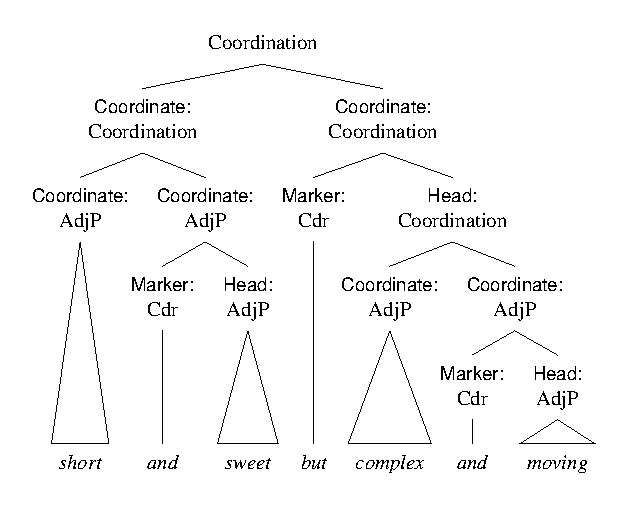
\includegraphics[width=0.9\linewidth]{figures/short and sweet but complex and moving.pdf}
    \caption{階層的等位接続：\mention{short and sweet but complex and moving}}\label{fig:coord-layered-ja}
\end{figure}

\subsection{特殊な等位接続}

特に興味深い等位接続の型は、比較構造に現れます。

\ea \label{ex:coord-comp-ja}
    \ea \gll He's as tall as {\ob}or taller than{\cb} his brother.\\
        he-である as 背が高い as or より背が高い than his 兄弟\\
    \glt \trans{彼は兄弟と同じくらい背が高いか、それより背が高い。}
    \ex \gll She writes more {\ob}but understands less{\cb} than before.\\
        she 書く-PRS より多く but 理解する-PRS より少なく than 以前\\
    \glt \trans{彼女は以前より多く書くが、理解は少なくなっている。}
    \z
\z
これらの構造では、等位要素と共有される要素の間に複雑な関係が含まれることがよくあります。その解釈には、等位接続と比較関係の両方を理解する必要があります。

\begin{tblsframedsymbol}{すばやい自己確認：複雑な構造}{test}
階層化した構造を分析できるか試してみましょう。
\begin{itemize}[noitemsep, leftmargin=*]
    \item \mention{I know that she left and he stayed} の中で、すべての従属化関係と等位接続関係を見つけてください。
    \item \mention{Both young and talented, she succeeded} の中で、相関的な標識と等位接続された形容詞を見つけてください。
    \item 次の構造を分析してください：\mention{He's taller than I thought but shorter than his brother}。
\end{itemize}
これらの複雑な型を理解すると、従属化と等位接続がどのように協働して意味を作るかが見えてきます。
\end{tblsframedsymbol}

\section{まとめ}

従属化と等位接続は、どちらも考えを結ぶという同じ仕事をしますが、反対の構造を使います。従属化は埋め込み、等位接続は結びます。よい文章はこの二つのバランスを取ります。学生がどの構造を使おうとしているのか、そしてどこで崩れているのかが分かれば、ただ「何か変だ」と感じるだけでなく、問題に名前をつけることができます。層が多すぎる、列挙しすぎている、等位接続詞で足りるところに従属接続詞を使っている、というようにです。
